\documentclass{scrartcl}
\usepackage{german}
\usepackage[utf8]{inputenc}
\usepackage[german]{babel}
\usepackage{amssymb}  % advanced mathematical symbold
\usepackage{graphicx} % using graphics
\usepackage{fancyhdr} % for the head of the page
\usepackage{lastpage} % makes page numbers work
\setlength{\parskip}{\medskipamount} % thats reasonable
\setlength{\parindent}{0pt}


%%%%%%%%%%%%%%%%%%%%%%%%
% Kopf- und Fusszeilen %
%%%%%%%%%%%%%%%%%%%%%%%%
\pagestyle{fancy}
\lhead{
    \begin{tabular}{ll}
        Felix Karg & 4342014\\
    \end{tabular}
}
\chead{Graphentheorie}
\rhead{
    \begin{tabular}{rr}
        \today{} \\
        Seite \thepage{} von \pageref{LastPage}
    \end{tabular}
}
\lfoot{}
\cfoot{}
\rfoot{}

%%%%%%%%%%%%%%%%%%%%%%%%
% Anfang des Dokuments %
%%%%%%%%%%%%%%%%%%%%%%%%
\begin{document}

\section*{Antworten zu Blatt 1}


\section*{Aufgabe 1}
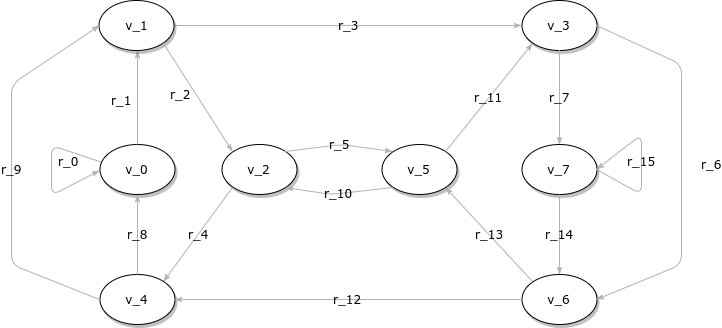
\includegraphics[width=14cm]{brown_graph.png}
\newline
\begin{itemize}
    \item[1)] $G' = (V', R', \alpha', \omega') $ mit \\
        $V' = {a, b, c, d, e, f, g, h}$ \\
        $R' = {r_0, r_1, .., r_{15}}$ \\
        $\alpha'(r_i) = v_{\lfloor i/2 \rfloor}$ \\
        $\omega'(r_i) = v_{i  mod  8}$ \\
        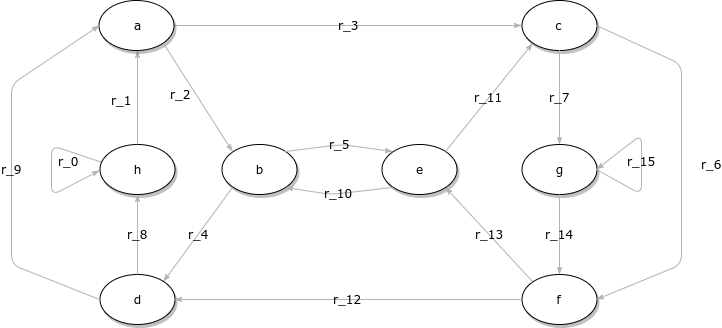
\includegraphics[width=14cm]{yellow_graph.png}
    \item[2)] Schlingen: $\{r_0, r_{15}\}$,
        Parallel: $\emptyset$,
        Antiparallel: $\{ (r_5, r_{10}) \}$.
    \item[3)]
        $\delta^+(v_6) = \{r_{12}, r_{13} \}$ (ausgehende relations),
        $\delta^+(v_7) = \{r_{14}, r_{15} \}$,
        $\delta^-(v_6) = \{r_{14}, r_{6} \}$ (eingehende relations),
        $\delta^-(v_7) = \{r_{7}, r_{15} \}$,
        $N^+(v_6) = \{ v_5, v_4\}$ (ausgehende nächste knoten),
        $N^+(v_7) = \{ v_7, v_6\}$,
        $N^-(v_6) = \{ v_3, v_7\}$ (eingehende, vorhergehende knoten),
        $N^-(v_7) = \{ v_3, v_7\}$,
    \item[4)] Alle knoten haben 4 eingehende sowie ausgehende Verbindungen,
        daher ist sowohl Minimal-, als auch Maximalgrad = 4.
    \item[5)] induzierter Subgraph von $v_0, v_2, v_4, v_6$: \\
        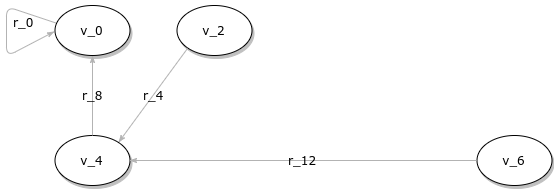
\includegraphics[width=10cm]{induced_sub_graph.png}
\end{itemize}

\section*{Aufgabe 2}
Ja, mit $\tau$ \\
$v_0 \leftrightarrow h$, \\
$v_1 \leftrightarrow a$, \\
$v_2 \leftrightarrow b$, \\
$v_3 \leftrightarrow c$, \\
$v_4 \leftrightarrow d$, \\
$v_5 \leftrightarrow e$, \\
$v_6 \leftrightarrow f$, \\
$v_7 \leftrightarrow g$, \\
sowie die relationen behaltend.

\section*{Aufgabe 3}
Graph: \\
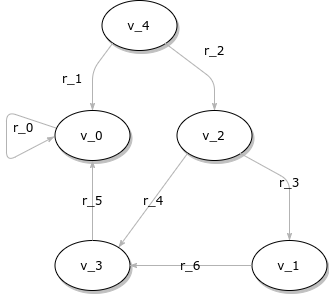
\includegraphics[width=7cm]{G_graph.png} \\
Partial und Subgraph (= Graph): \\
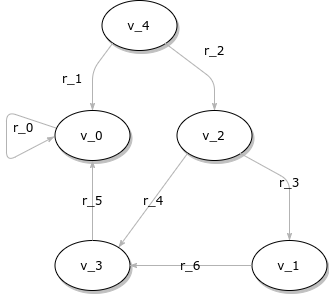
\includegraphics[width=7cm]{G_graph.png} \\
Weder Partial noch Subgraph davon: \\
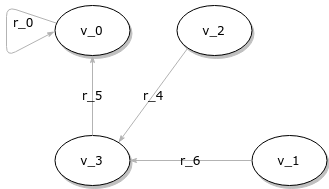
\includegraphics[width=7cm]{no_partial_sub_graph.png}



\end{document}


Beispiel für Text, der aus einem Terminal kopiert wurde:

\begin{verbatim}
osswald@tfpool17 / $ df -h
Filesystem                           Size  Used Avail Use% Mounted on
/dev/sda4                            375G   41G  316G  12% /
dev                                  3.9G     0  3.9G   0% /dev
run                                  3.9G  480K  3.9G   1% /run
tmpfs                                3.9G     0  3.9G   0% /dev/shm
\end{verbatim}

Aufzählungen sind mit \verb_enumerate_ möglich:
\begin{enumerate}
\item Erster Punkt
\item Zweiter Punkt
\item Dritter Punkt
\end{enumerate}

\subsection*{Aufgabe 2}

Mathematische Formeln:
\begin{equation}\label{gauss}
    \sum_{i=1}^{n} i = \frac{n(n+1)}{2}
\end{equation}


Formel \ref{gauss} wird auch \emph{Gaußsche Summenformel} genannt.

Formeln können auch im Text eingebunden werden, z.B. $E = mc^{2}$.

\subsection*{Aufgabe 3}

Tabellen können mit \verb_tabular_-Umgebungen eingegeben werden:

\begin{center}
\begin{tabular}{l|l|l}
Datei             & Dateirechte        & Größe   \\
\hline
dokument.txt      & \verb_-rw-r--r--_  & 300 KB  \\
programm.exe      & \verb_-rwxr-x---_  & 450 KB  \\
mein\_verzeichnis & \verb_drwxr-xr-x_  & ---     \\
\end{tabular}
\end{center}

\end{document}


